\documentclass[a4paper]{article}
\usepackage[14pt]{extsizes}
\usepackage[T2A]{fontenc}
\usepackage[utf8]{inputenc}
\usepackage[russian]{babel}
\usepackage{setspace,amsmath}
\usepackage{graphicx}
\usepackage{epigraph} 
\usepackage{csquotes} 
\usepackage[unicode, pdftex]{hyperref} 
\usepackage{amssymb} 
\usepackage{caption}
\usepackage{amsthm} 
\usepackage{wrapfig}
\usepackage[left=15mm, top=10mm, right=10mm, bottom=15mm, nohead, footskip=10mm]{geometry} 
\RequirePackage{caption}
\DeclareCaptionLabelSeparator{d}{}
\captionsetup{justification=centering,labelsep=d}
\usepackage{multirow}

\begin{document}
\title{\textbf{Лабораторная работа 1.4.5}

\

Изучение колебаний струны

\
}
\author{И. М. Артёмов}
\date{\today}
\maketitle
\noindent
\textbf{Цель работы}: изучить поперечные стоячие волны на тонкой натянутой струне; измерить собственные частоты колебаний струны и проверить условие образования стоячих волн; измерить скорость распространения поперечных волн на струне и исследовать её зависимость от натяжения струны.

\

\noindent
\textbf{Оборудование}: закрепленная на станине стальная струна, набор грузов, электромагнитные датчики, звуковой генератор, двухканальный осциллограф, частотомер.

\section*{1. Теоретическое введение}
В работе изучаются поперечные колебания стальной гитарной струны, натянутой горизонтально и закрепленной между двумя неподвижными зажимами. Так как поперечные размеры струны много меньше её длины, то напряжение в струне может быть направлено только \textit{вдоль неё}. В натянутой струне возникает \textit{поперечная упругость}, то есть способность сопротивляться всякому изменению формы, происходящему без изменения объёма. При вертикальном смещении произвольного элемента струны, возникают силы, действующие на соседние элементы, и в результате вся струна приходит в движение в вертикальной плоскости, т.е. возбуждение «бежит» по струне. Передача возбуждения представляет собой \textit{поперечные бегущие волны}, распространяющиеся с некоторой скоростью в обе стороны от места возбуждения. В ненатянутом состоянии струна не обладает свойством поперечной упругости, и поперечные волны на ней невозможны.

\subsection*{1.1. Уравнение волны на струне}
Рассмотрим гибкую однородную струну, в которой создано натяжение T, и получим дифференциальное уравнение, описывающее её малые
поперечные свободные колебания. Отметим, что, если струна расположена
горизонтально в поле тяжести, величина T должна быть достаточна для
того, чтобы в состоянии равновесия струна не провисала, т.е. сила натяжения должна существенно превышать вес струны.

\noindent
Направим ось $x$ вдоль струны в положении равновесия. Форму волны будем описывать функцией $y(x,t)$, определяющей вертикальное смещение $y$ струны в данной точке в любой момент времени $t$. Рассмотрим малый элемент $dm$ струны. Так как амплитуда колебаний невелика, то можно пренебречь добавочным напряжением, возникающим из-за удлинения элементов струны и считать силу $T$ натяжения нити постоянной по её длине. Также можно считать углы отклонения $\alpha$ струны от оси $x$ малыми. В итоге по 2 закону Ньютона в проекциях на ось $y$ для элемента получим:
\begin{figure}
\center{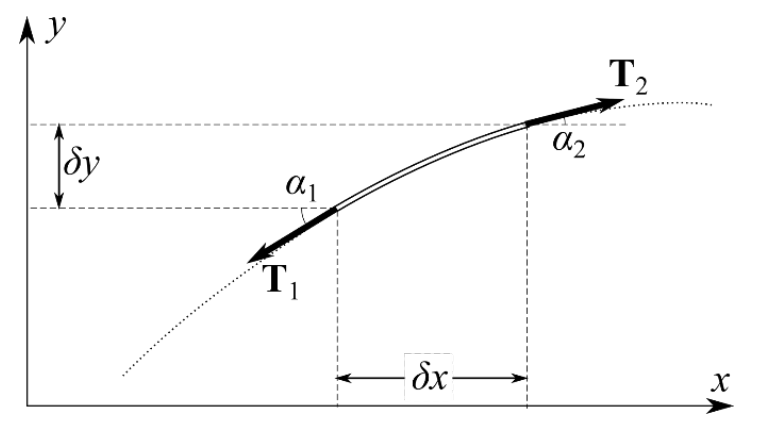
\includegraphics[scale=0.9]{рис 1.png}}
\caption{. \textit{К выводу уравнения колебаний струны}}
\end{figure}
\begin{equation}
T \alpha_2 - T \alpha_1 \approx \frac{\partial^2 y}{\partial t^2} dm
\end{equation}
Учтём, что в ненатянутом положении длина элемента равна $\delta x$, то есть $dm = \rho \delta x$, где $\rho$ - линейная плотность нити в ненатянутом состоянии. Тогда, учитывая, что $\alpha = \partial y/\partial x$, получим:
\begin{equation}
T\delta \alpha = \frac{\partial^2 y}{\partial t^2} \rho \delta x \Rightarrow \frac{\partial^2 y}{\partial t^2} = \frac{T}{\rho} \frac{\partial^2 y}{\partial x^2} = u^2 \frac{\partial^2 y}{\partial x^2} \quad \left(u = \sqrt{\frac{T}{\rho}}\right)
\end{equation} 
\fbox{%
\begin{minipage}{0.3 \linewidth} 
\centering
$\frac{\partial^2 y}{\partial t^2} = u^2 \frac{\partial^2 y}{\partial x^2} \quad (*) $
\end{minipage}}
- \textit{уравнение свободных малых поперечных колебаний в струне}. Оно также называется волновым уравнением.

\subsection*{1.2. Бегущие волны}
Заметим, что произвольная функция вида $y(x,t) = f(x-ut)$ является решением волнового уравнения $(*)$. Действительно, обозначим $\psi(x,t) = x-ut$. Тогда 
\begin{equation}
y(x, t) = f(\psi(x,t)) \Rightarrow \frac{\partial y}{\partial t} = \frac{df}{d\psi} \frac{\partial \psi}{\partial t} \Rightarrow \frac{\partial^2 y}{\partial t^2} = \frac{\partial \psi}{\partial t} \left(\frac{d^2 f}{d\psi^2} \frac{\partial \psi}{\partial t}  \right) + \frac{df}{d\psi} \frac{\partial^2 \psi}{\partial t^2}
\end{equation}
Аналогично:
\begin{equation}
\frac{\partial^2 y}{\partial x^2} = \frac{\partial \psi}{\partial x} \left(\frac{d^2 f}{d\psi^2} \frac{\partial \psi}{\partial x}  \right) + \frac{df}{d\psi} \frac{\partial^2 \psi}{\partial x^2}
\end{equation}
\begin{flalign*}
\text{Учитывая, что } \ \frac{\partial \psi}{\partial t} = u, \ \frac{\partial^2 \psi}{\partial t^2} = 0, \ \frac{\partial \psi}{\partial x} = 1 , \ \frac{\partial^2 \psi}{\partial x^2} = 0 \text{, получим:} &&
\end{flalign*}
\begin{equation}
\frac{\partial^2 y}{\partial t^2} = u^2 \frac{d^2 f}{d\psi^2} = u^2 \frac{\partial^2 y}{\partial x^2}
\end{equation}

\noindent
Заметим теперь, что если в уравнении $y(x, t) = f(\psi(x,t))$ положить $\psi = const$, то получим: $dx/dt = u$, то есть возмущение струны движется поступательно со скоростью $u$ вдоль оси $x$.

\noindent
Общее же решение волнового уравнения представимо в виде суперпозиции двух волн произвольной формы, бегущих вдоль оси $x$ со скоростями $\pm u$:
\begin{equation}
y(x,t) = f_1(x-ut) + f_2(x+ut)
\end{equation}
Вид функций $f_1$ и $f_2$ в данной конкретной задаче определяется из начальных и граничных условий.
В данной работе будут изучаться \textit{гармонические волны}:
\begin{equation*}
y(x,t) = a \cos\left[k(x - ut)\right] + b \cos\left[k(x+ut)\right] = 
\end{equation*}
\begin{equation}
= a\cos\left(\omega t - kx\right) + b\cos\left(\omega t + kx\right)
\end{equation}
Здесь $\omega$ - циклическая частота колебаний, а $k = \frac{\omega}{u} = \frac{2\pi}{\lambda}$ - \textit{пространственная частота} волны. ($\lambda$ - длина волны).

\subsection*{1.3. Собственные колебания струны. Стоячие волны} 

\noindent
Найдем вид свободных колебаний струны с \textit{закрепленными концами}. Пусть струна закреплена в точках $x = 0$ и $x = L$. Тогда из условия $y(0, t) = 0 \ (\forall t)$, получим:
\begin{equation}
a \cos(\omega t) + b \cos(\omega t) = 0 \Rightarrow a = -b
\end{equation} 
Тогда:
\begin{equation}\label{eq9}
y(x,t) = a(\cos(\omega t - k x) - \cos(\omega t + k x)) = 2 a \sin{kx} \cdot \sin{\omega t}
\end{equation}

\noindent
Нетрудно видеть, что данная волна получается в результате суперпозиции двух гармонических бегущих навстречу друг другу волн с равными амплитудами. Такая волна называется \textit{стоячей}. Вся струна колеблется с циклической частотой $\omega$. При этом амплитуда колебаний распределена по струне по закону: $y_m(x) = 2 a \sin{kx}$. В точках, где $\sin{kx} = 1$, амплитуда колебаний максимальна (\textit{пучности волны}). Точки, у которых $\sin{kx} = 0$ не колеблются вовсе (\textit{узлы волны}). Точки струны между двумя соседними узлами всегда колеблются в одной фазе, то есть в любой момент времени их скорости сонаправлены.

\noindent
Используем второе граничное условие $y(L, t) = 0 \ (\forall t)$:
\begin{equation}
\sin{kL} = 0 \Rightarrow kL = \pi n, \quad n \in \mathbb {N} 
\end{equation}
Тогда:
\begin{equation}
\lambda_n = \frac{2L}{n}, \quad n \in \mathbb{N}
\end{equation}
Как видно, параметр $n$ определяет число полуволн (то есть пучностей), которые умещаются на струне. Так как длина волны однозначно связана с её частотой, то струна может колебаться только с определёнными частотами:
\begin{equation}\label{eq12}
\nu_n = \frac{u}{2L} n
\end{equation}
Спектр собственных частот $\nu_n$ колебаний струны зависит только от её натяжения, линейной плотности и длины и, в случае малых гармонических колебаний, не зависит от модуля Юнга материала струны.

\subsection*{1.4. Возбуждение колебаний струны. Резонанс} При колебаниях реальной струны всегда имеет место потеря энергии. Поддержание незатухающих
колебаний в струне может осуществляться точечным источником, в качестве которого в данной работе используется электромагнитный вибратор. 
Для эффективной раскачки колебаний используется явление резонанса - необходимо, чтобы вынуждающая частота $\nu$ вибратора совпала с одной из собственных частот $\nu_n$ струны. Тогда в любой момент времени потери энергии будут компенсироваться поступающей от воздбудителя колебаний энергией, процесс становится стационарным и можно наблюдать стоячие волны.

\noindent
Также стоит отметить, что в идеальном случае поток энергии вдоль стоячей волны отсутствует (в каждом участке между узлами кинетическая энергия переходит в потенциальную и наоборот). Однако, энергия от вибратора должна каким-то образом доходить до удалённых от него частей струны, поэтому в реальности помимо стоячей волны, есть ещё и малая бегущая компонента, которая и переносит энергию источника. Если потери энергии за период малы по сравнению с запасом колебательной энергии в струне, то искажение стоячих волн бегущей волной не существенно — наложение бегущей волны малой амплитуды на стоячую визуально приводит к незначительному «размытию» узлов (амплитуда колебаний в узлах совпадает с амплитудой бегущей компоненты волны).

\noindent
Для достижения максимальной раскачки колебаний, необходимо располагать возбуждающий контакт вблизи узловый точки (но не строго в ней). Действительно, предположим, что вибратор способен раскачать соответствующий элемент струны до амплитуды $A$. Если $x_0$ - расстояние от него до пучности, то из формулы \eqref{eq9}:
\[A = 2a \sin{kx_0} \Rightarrow a = \frac{A}{2\sin{kx_0}} \]
Отсюда видно, что расстояние $x_0$ следует устремлять к нулю.

\noindent
Наконец отметим, что в ходе работы необходимо добиться того, чтобы колебания были \textit{линейно поляризованы}, то есть чтобы струна колебалась в одной плоскости. Также необходимо обеспечить малость амплитуды колебаний - в противном случае волновое уравнение $(*)$ будет неприменимо.

\section*{2. Описание экспериментальной установки}
Схема установки приведена на рис. 2. Стальная гитарная струна 1 закрепляется в горизонтальном положении между двумя стойками с зажимами 2 и 3, расположенными на массивной станине 4. Один конец струны
закреплен в зажиме 2 неподвижно. К противоположному концу струны, перекинутому через блок, прикреплена платформа с грузами 5, создающими
натяжение струны. Зажим 3 можно передвигать по станине, устанавливая
требуемую длину струны. Возбуждение и регистрация колебаний струны
осуществляются с помощью электромагнитных датчиков (вибраторов),
расположенных на станине под струной. Электромагнитный датчик 6 подключен к звуковому генератору 7 и служит для возбуждения колебаний
10
струны, частота которых измеряется с помощью частотомера 10 (в некоторых установках частотомер встроен в генератор). Колебания струны регистрируются с помощью электромагнитного датчика 8, сигнал с которого
передается на вход осциллографа 9. Разъёмы, через которые датчики с помощью кабелей соединяются с генератором и осциллографом, расположены на корпусе станины.
\begin{figure}
\center{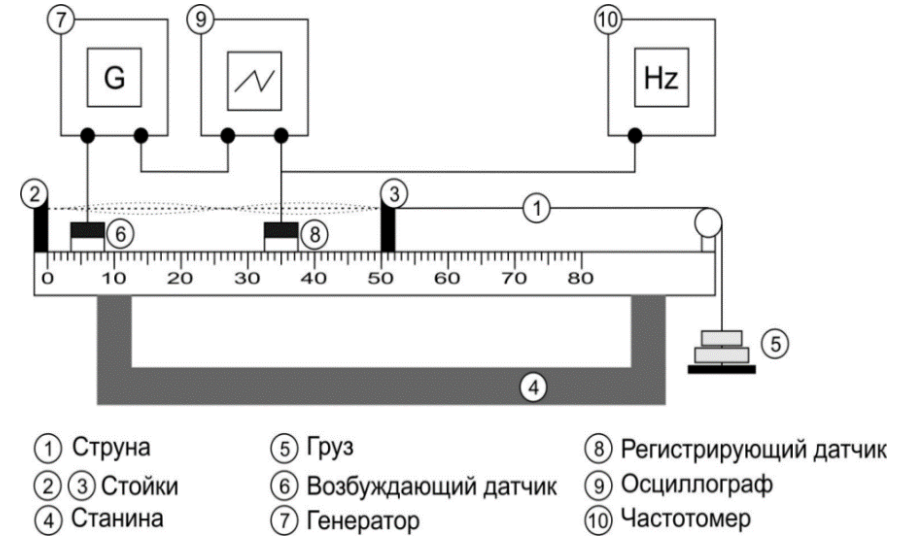
\includegraphics[scale=0.8]{рис 2.png}}
\caption{. \textit{Экспериментальная установка}}
\end{figure}

\section*{3. Ход работы.}
\begin{itemize}
\item[\textbf{1. }] Освобождаем зажим струны на стойке \textbf{3} и устанавливаем начальную длину $L = $ (это рекомендованное значение, указанное на установке). Подвешиваем $N_1 = 2$ грузика к нити массами: $m_1 = 487.4$ г и $m_2 = 453.4$ г. Зажимаем струну в стойке \textbf{3}. Располагаем возбуждающий датчик \textbf{6} рядом с неподвижной стойкой \textbf{2}. 
\item[\textbf{2. }] Проведём предварительные расчёты.	Так как масса подвеса \textbf{5} равна $M_{sup} = 115.1$ г, то сила натяжения нити: $T = (M_{sup} + m_1+m_2)g$. Линейная плотность струны указана на установке: $\rho = 568.4$ мг/м. Тогда скорость распространения волн в струне:
\begin{equation}
u = \sqrt{\frac{\left(M_{sup} + \sum\limits_{i=1}^{N_1}m_i \right)g}{\rho}} \approx 142 \frac{\text{м}}{{\text{с}}}
\end{equation}
Длину струны измеряем линейкой: $L = (49.00 \pm 0.05)$ см. Рассчитаем частоту \textit{основной гармоники} струны по формуле \eqref{eq12}
\[\nu_1 = \frac{1}{2L} u \approx 145 \text{ Гц} \]
Зная значения $u$ и $L$, можно предварительно рассчитать значения остальных гармоник по формуле \eqref{eq12}.
\item[\textbf{3. }] Включим в сеть звуковой генератор, установим на нём синусоидальный тип сигнала. Установим регистрирующий датчик \textbf{8} в центре под струной (в месте пучности). Убедиждаемся, что сигнал с выхода генератора подаётся на возбуждающий датчик 6. Устанавливаем на генераторе рассчитанную частоту $\nu_1$
\item[\textbf{4. }] Медленно изменяя частоту генератора в пределах $\nu_1 \pm 5$ Гц, добиваемся возбуждения стоячей волны с максимальной амплитудой. Записываем частоту, выдаваемую генератором (табл.1).
\item[\textbf{5. }] Увеличим частоту генератора в 2 раза и аналогичным образом определим частоту $\nu_2$, при которой амлпитуда колебаний достигает максимума. Проведём такое же измерение для третьей гармоники. Результат - в табл. 1

\begin{table}[h!]
\centering
\begin{minipage}{0.5\linewidth}
\centering
\begin{tabular}{|c|c|c|}
\hline
$\nu_1$, Гц & $\nu_2$, Гц & $\nu_3$, Гц \\ \hline
132.0       & 270.0       & 404.0       \\ \hline
\end{tabular}
\caption{}
\end{minipage}
\end{table}
\item[\textbf{6. }] Изменим амплитуду сигнала генератора так, чтобы при колебаниях струна не касалась регистрирующего датчика \textbf{8}. Убедимся, что сигнал колебаний струны с датчика \textbf{8} подаётся на вход канала 2 осциллографа, а на вход канала 1 подаётся опорный сигнал с генератора на частоте возбуждения струны.
Включим осциллограф в сеть и проверим его настройку. Выведем на экран сигнал с регистрирующего датчика. 

\noindent
Подстроим частоту $\nu$ генератора так, чтобы она была близка к рассчитанной частоте $\nu_1$ основной гармоники. Добьёмся, чтобы амплитуда регистрируемого сигнала была максимальной. Окончательное значение частоты генератора:
\[\nu_1 = 134.6 \text{ Гц} \]
\item[\textbf{7. }] Проведём измерения частот ещё 4 нечётных гармоник. Регистрирующий датчик стоит оставлять под струной. Результаты - в табл. 2

\begin{table}[]
\begin{minipage}{0.19 \linewidth}
\centering
\begin{tabular}{|c|c|}
\hline
$n$  & $\nu_n$, Гц \\ \hline
1  & 134.6     \\ \hline
2  & 271.2     \\ \hline
3  & 405.3     \\ \hline
4  & 543.6     \\ \hline
5  & 681.9     \\ \hline
6  & 819.3     \\ \hline
7  & 957.1     \\ \hline
8  & 1096.0    \\ \hline
9  & 1238.4    \\ \hline
10 & 1378.0    \\ \hline
\end{tabular}
\caption{}
\end{minipage}
\begin{minipage}{0.19 \linewidth}
\centering
\begin{tabular}{|c|c|}
\hline
$n$ & $\nu_n$, Гц \\ \hline
1   & 161.5     \\ \hline
2   & 325.0       \\ \hline
3   & 488.7     \\ \hline
4   & 653.6     \\ \hline
5   & 811.9     \\ \hline
6   & 982.4     \\ \hline
7   & 1149.0      \\ \hline
8   & 1313.0      \\ \hline
9   & 1479.0      \\ \hline
10  & 1645.0      \\ \hline
\end{tabular}
\caption{}
\end{minipage}
\begin{minipage}{0.19 \linewidth}
\centering
\begin{tabular}{|c|c|}
\hline
$n$ & $\nu_n$, Гц \\ \hline
1   & 186.7     \\ \hline
2   & 373.5     \\ \hline
3   & 563.0       \\ \hline
4   & 750.4     \\ \hline
5   & 940.3     \\ \hline
6   & 1129.6    \\ \hline
7   & 1317.5    \\ \hline
8   & 1505.0      \\ \hline
9   & 1695.0      \\ \hline
10  & 1881.0      \\ \hline
\end{tabular}
\caption{}
\end{minipage}
\begin{minipage}{0.19 \linewidth}
\centering
\begin{tabular}{|c|c|}
\hline
$n$ & $\nu_n$, Гц \\ \hline
1   & 201.4     \\ \hline
2   & 404.3     \\ \hline
3   & 607.5     \\ \hline
4   & 810.4     \\ \hline
5   & 1013.5    \\ \hline
6   & 1215.0      \\ \hline
7   & 1418.0      \\ \hline
8   & 1622.0      \\ \hline
9   & 1825.0      \\ \hline
10  & 2031.0      \\ \hline
\end{tabular}
\caption{}
\end{minipage}
\begin{minipage}{0.19 \linewidth}
\centering
\begin{tabular}{|c|c|}
\hline
$n$ & $\nu_n$, Гц \\ \hline
1   & 223.0       \\ \hline
2   & 444.0       \\ \hline
3   & 667.5     \\ \hline
4   & 891.6     \\ \hline
5   & 1113.0      \\ \hline
6   & 1338.0      \\ \hline
7   & 1559.0      \\ \hline
8   & 1783.0      \\ \hline
9   & 2008.0      \\ \hline
10  & 2233.0          \\ \hline
\end{tabular}
\caption{}
\end{minipage}
\end{table}
\begin{table}
\centering
\begin{minipage}{0.49\linewidth}
\centering
\begin{tabular}{|c|c|c|c|}
\hline
\textnumero \ опыта            &\textnumero \ груза & $m_i$, г & $T$, Н                \\ \hline
\multirow{2}{*}{1} & 1     & 487.4    & \multirow{2}{*}{10.3} \\ \cline{2-3}
                   & 2     & 453.4    &                       \\ \hline
2                  & 3     & 483.4    & 15.1                  \\ \hline
3                  & 4     & 491.9    & 19.9                  \\ \hline
4                  & 5     & 334.3    & 23.2                  \\ \hline
5                  & 6     & 494.6    & 28.0                    \\ \hline
\end{tabular}
\caption{}
\end{minipage}
\begin{minipage}{0.49\linewidth}
\centering
\begin{tabular}{|c|c|c|}
\hline
N опыта & $u$, м/с & $\sigma_u$, м/с \\ \hline
1       & 135.3    & 0.3             \\ \hline
2       & 161.6    & 0.3             \\ \hline
3       & 184.7    & 0.2             \\ \hline
4       & 199.0    & 0.2             \\ \hline
5       & 218.8    & 0.3             \\ \hline
\end{tabular}
\caption{}
\end{minipage}
\end{table}
\item[\textbf{8. }] Измерим 5 частот нечётных гармоник. Заметим, что теперь посередине струны всегда находится узел волны, поэтому регистрирующий датчик стоит сместить в сторону пучности. Для $n$, не делящихся на 4, можно располагать датчик на расстоянии $L/4 \approx 12.3$ см от стойки $3$, для $n=4$ расположим датчик на расстоянии $3L/8 \approx 18.4$ см, для $n=8$ - на расстоянии $15L/16 \approx 21.4$ см. Результаты - в табл. 2
\item[\textbf{9. }] Повторим пункты 7 и 8 ещё для четырёх значений $T$. $T$ будем изменять, подвешивая всё большее число грузов к нити. Результаты - в табл. 3, 4, 5, 6. В табл. 7 представлены значения масс грузов, подвешенных в каждом из пяти опытов и силы натяжения нитей.
\item[\textbf{10. }] Построим графики зависимостей $\nu_n(n)$ для каждого из пяти опытов и аппроксимируем их линейной функцией по МНК. Результаты - на рис. 3. Зная угловые коэффициенты $\beta$ этих зависимостей, определим скоросоть распространения волн в струне в каждом случае, как:
\[u = 2\beta L \]
Результаты - в табл. 8. Погрешность измерения $u$ считалась, как:
\[\sigma_u = u \sqrt{\left(\frac{\sigma_{\beta}}{\beta}\right)^2+\left(\frac{\sigma_L}{L}\right)^2}\]




\begin{figure}
\center{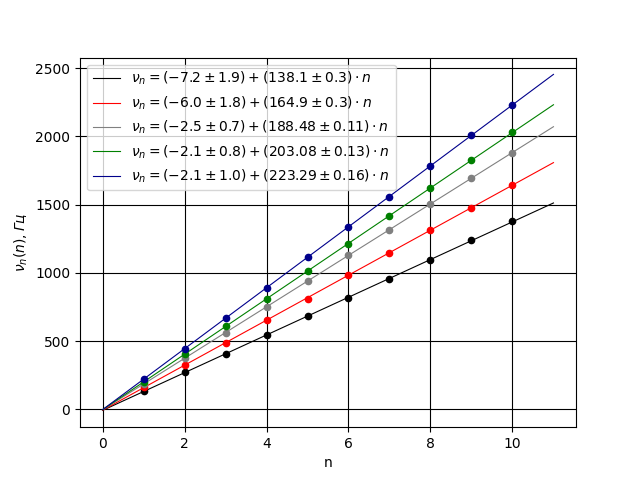
\includegraphics[scale=0.95]{рис 3.png}}
\caption{\textit{. Графики зависимостей $\nu_n(n)$ и их аппроксимация линейной функцией по МНК}}
\end{figure}
\begin{figure}
\center{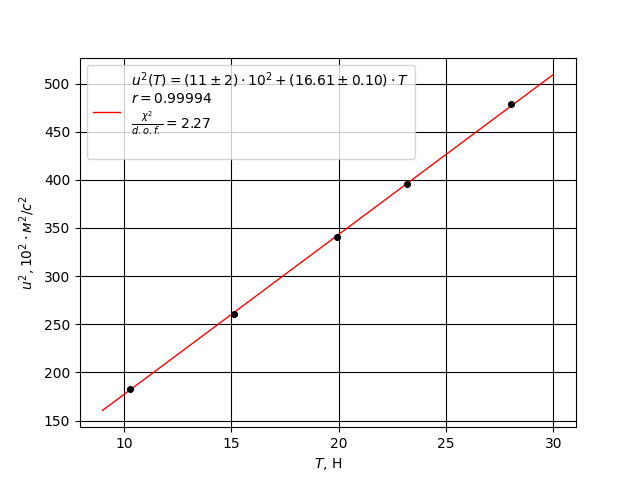
\includegraphics[scale=0.95]{рис 4.png}}
\caption{. \textit{График зависимости $u^2(T)$ и его аппроксимация линейной функцией по хи-квадрат}}
\end{figure}

\item[\textbf{11. }] Построим график зависимости $u^2(T)$. Результат - на рис. 4. Погрешность измерения $u^2$ считалась по формуле:
\[\sigma_{u^2} = 2 u \sigma_u \]
Аппроксимируем график линейной функцией методом хи-квадрат. Получим, что если $u^2(T) = a + bT$, то:
\[a = (11 \pm 2)\cdot 10^2 \ \frac{\text{м}^2}{\text{с}^2} \quad ; \quad b = (16.61 \pm 0.10) \cdot 10^2 \  \frac{\text{м}}{\text{кг}} \quad; \quad r \approx 0.99994 \quad; \quad \frac{\chi^2}{d.o.f.} \approx 2.27\]
Отсюда получим значение линейной плотности струны:
\[\rho = \frac{1}{b} \approx (602 \pm 4) \ \frac{\text{мг}}{\text{м}} \quad ; \quad \varepsilon_{\rho} = \frac{\sigma_{\rho}}{\rho} \approx 7 \cdot 10^{-3} \ \% \quad ; \quad \left(\sigma_{\rho} = \frac{\sigma_b}{b^2}\right)\]
\end{itemize}

\section*{4. Вывод}
В работе были изучены поперечные стоячие волны на тонкой натянутой струне, были измерены собственные частоты её колебаний, измерена скорость распространения волн в струне и линейная плотность струны. Экспериментальные графики зависимостей $\nu_n(n)$ и $u^2(T)$ хорошо ложатся на аппроксимирующие прямые, но эти прямые не проходят через начало координат. Однако отклонение аппроксимирующих прямых от начала координат по оси ординат мало ($\sim 1\%$) по сравнению с значениями ординат экспериментальных точек. Отличие измеренного значения линейной плотности струны от указанного на установке составляет $6 \%$. Само значение $\rho$ измерено с достаточно высокой точностью $\varepsilon_{\rho} = 7 \cdot 10^{-3} \ \%$. Отличие $\rho$ от указанного на установке значения более, чем на погрешность, может быть связано с:
\begin{itemize}
\item[1) ] Неточностью определения собственных частот $\nu_n$ из-за возникновения нелинейных эффектов при резонансе, и, как следствие, неточностью в определении скорости распространения $u$ волны в струне.
\item[2) ] Неучтением погрешностей измерения собственных частот.
\item[3) ] Недостаточным количеством экспериментальных точек на графике $u^2(T)$, то есть недостаточным количеством опытов по измерению собственных частот струны в зависимости от силы натяжения нити $T$.
\end{itemize}


\end{document}